\section{Experiments}

\paragraph{A metric to determine when MTL performs better STL.}
\begin{table}
\begin{center}
  \begin{tabular}{c c c}
  \toprule
    {\bf Threshold}  & {\bf Precision} &  {\bf Recall} \\
    \midrule
    0.0 & 0.596 & 1.000 \\
    0.1 & 0.756 & 0.388 \\
    0.2 & 0.919 & 0.065 \\
    0.3 & 1.000 & 0.004 \\	
  \bottomrule
  \end{tabular}
\end{center}
\caption{Ablation study on when should use MTL via different source/target task accuracy. Note: source task size range [500, 1500], target task size: 1000}
\label{tab:mtl_better_than_stl}
\end{table}


\paragraph{When should we align task covariances in MTL.}
\begin{figure}
	\centering
	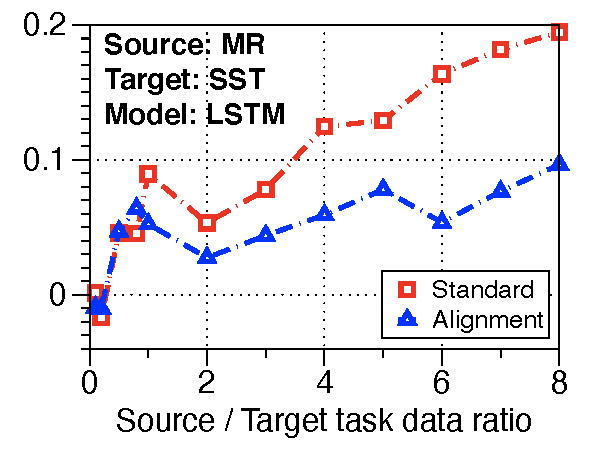
\includegraphics[width=0.5\textwidth]{figures/ratio_alignment_mr_sst_lstm.pdf}
	\caption{Covariate shift experiment.}
\end{figure}

\begin{figure}
	\centering
	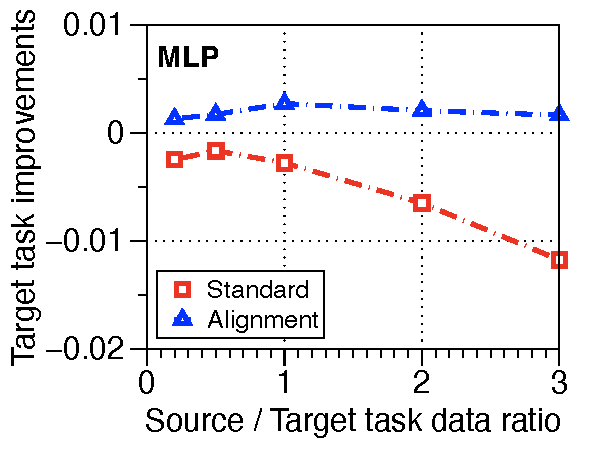
\includegraphics[width=0.5\textwidth]{figures/ratio_alignment_mlp.pdf}
	\caption{Covariate shift experiment.}
\end{figure}
